\begin{frame}
\frametitle{Introduction }
\begin{block}{}
\[ 
F(x) = \int_\Omega \norm{x - y}^{2n} e^{-\frac{\norm{x - y}^2}{\delta}} f(y) \, d\Omega
 \] 
\end{block}

\end{frame}


\begin{frame}
\frametitle{Introduction }
\framesubtitle{Kernels}
\begin{block}{}

* Thermal Sciences 

* Fluid Mechanics

* Neuroscience


\end{block}

\end{frame}

\begin{frame}	
\frametitle{Introduction }
\framesubtitle{Data-intensive Applications}

\begin{columns}
\begin{column}{.5\textwidth}
 
            \begin{center} Moderate \textbf{Re} blood flow \includegraphics[width = 1.5in]{Rbcflow.PNG} \csy{Pozrikidis, 2006}\end{center}

  	\begin{center} Cardiac mechanics 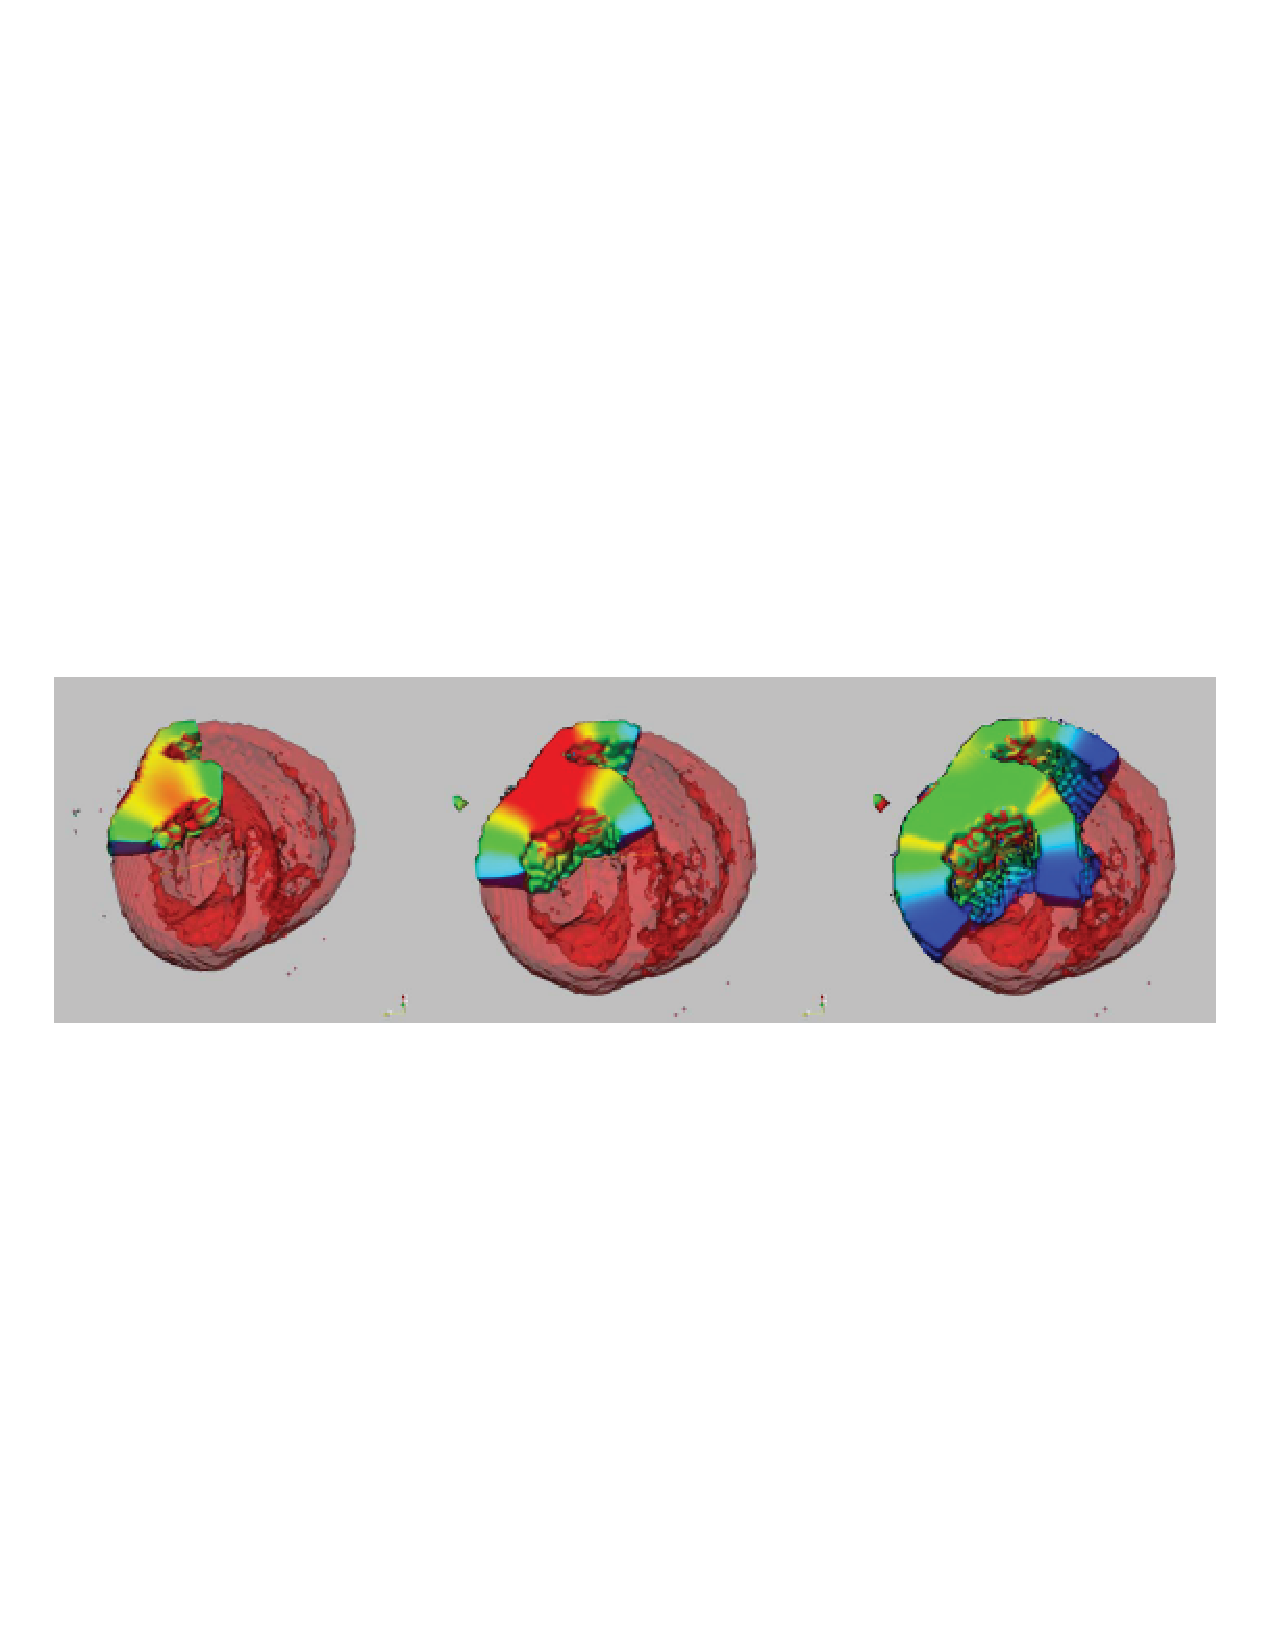
\includegraphics[width = 2in]{heart} \csy{Adavani-Biros,2008}\end{center}

\end{column}
\begin{column}{.5\textwidth}
    \begin{center}Design of MEMS \includegraphics[width = 1.6in]{resonator.jpg} \csy{White's group (MIT)}\end{center}
    
\begin{block}{Common challenges}
\begin{itemize}
 \item Moving geometries
 \item Multi-scale phenomena
 \item
 \item
\end{itemize}
\end{block}

\end{column}
\end{columns}
\end{frame}

\begin{frame}
\frametitle{Introduction }
\framesubtitle{Related Work}
\begin{block}{Sequential}

\end{block}

\begin{block}{Parallel}

\end{block}
\end{frame}

